\documentclass{article}

% these packages let you do math
\usepackage{amsmath}
\usepackage{amssymb}

% we need these packages for fancy R tables
\usepackage{booktabs}
\usepackage{float}
\usepackage{colortbl}
\usepackage{xcolor}

% these packages play with the spacing/margins of the document. Uncomment the commands on lines 16 and 17 to see what they do.
\usepackage{a4wide}
\usepackage{setspace}
\usepackage{geometry}
\usepackage{parskip}
%\doublespacing
%\geometry{margin=1.5in}

% this package helps us with including images. Setting the graphics path makes it easier to refer to things in the \includegraphics command.
\usepackage{graphicx}
\graphicspath{ {../figures/} }

% make some hyperlinks using the \href command
\usepackage{hyperref}
\hypersetup{
    colorlinks=true,
    linkcolor=black,
    urlcolor=blue
}

% set the author, title, and date of the document. \maketitle adds it to the document.
\author{Taylor Neal}
\title{My Paper on NLSY97 Data}
\date{Sping 2022}

\begin{document}
\maketitle

\section{Introduction}

In this report, we will utilize publicly available NLS data (from the National Longitudinal Survey of Youth 1997) to analyze incarceration rates in the year 2002. This exercise will seek to describe patterns revealed when examining this data across both race and gender. Incarceration status for each individual in the survey is provided on a monthly basis. Our primary variable of interest will be mean number of months spent incarcerated in 2002.

\newpage

\section{Results and Discussion}


\begin{figure}[H]
    \begin{center}
        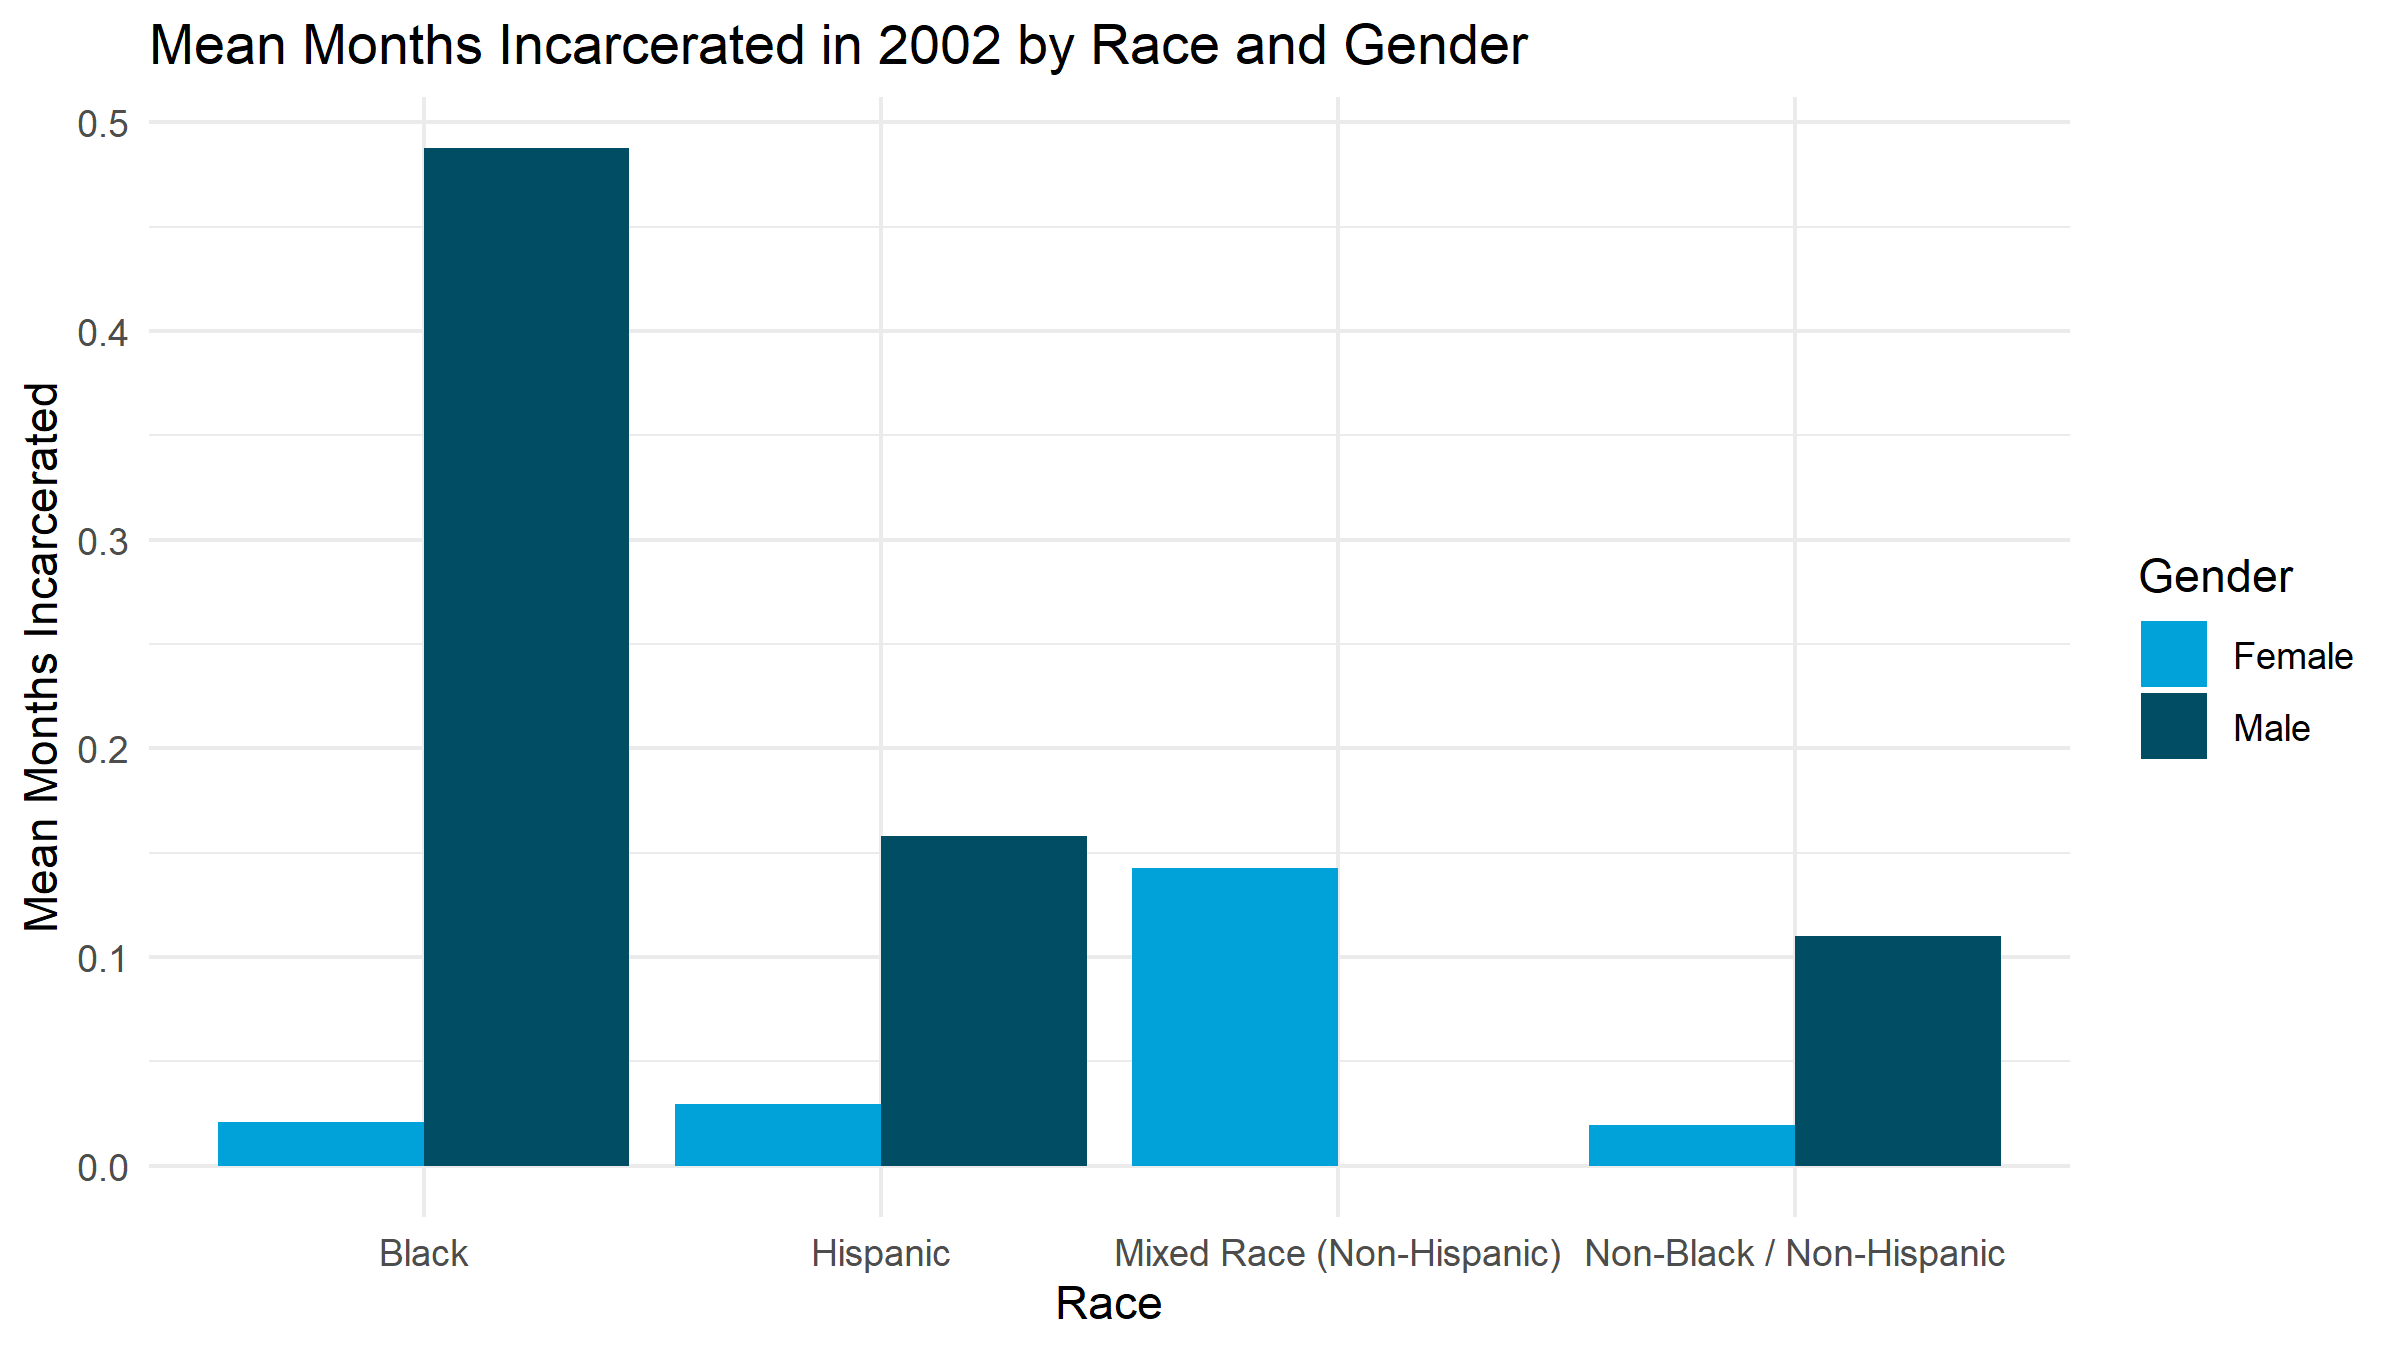
\includegraphics[width=.85\textwidth]{incarceration_by_racegender}
    \end{center}
    \caption{Mean Number of Months Incarcerated in 2002 by Race and Gender}
    \label{fig:graph}
\end{figure}


The most striking aspect of the figure above is the relative height of the bar for black men. For individuals included in the survey, mean number of months incarcerated in 2002 was over twice as high for black men compared to the next highest race/gender (Hispanic men). The mean number of months black women spent incarcerated was dramatically lower than their male counterparts. This is generally true for the male/female comparisons in this data (with the exception of Mixed Race Non-Hispanic), but the distinction is greatest in the case of black women and men. An additional point to make is the Mixed Race (Non-Hispanic) bars for men and women both seem inconsistent when compared to the rest of the data. The female bar is significantly larger than the next largest bar for women. And the mean number of months men spent incarcerated shows as zero. This could indicate that mixed race men are incorrectly being coded as women in the data. Alternatively, this observed behavior might be due to under-representation of Mixed Race (Non-Hispanic) individuals in the survey making our observations prone to outlines. Note the table below displays numerical values for the figure on the prior page.


\begin{table}[H]

\caption{\label{tab:tab:summarystats}Mean Months Incarcerated in 2002 by Race and Gender}
\centering
\begin{tabular}[t]{lrrrr}
\toprule
Gender & Black & Hispanic & Mixed Race Non Hispanic & Non Black Non Hispanic\\
\midrule
\cellcolor{gray!6}{Female} & \cellcolor{gray!6}{0.0211268} & \cellcolor{gray!6}{0.0298013} & \cellcolor{gray!6}{0.1428571} & \cellcolor{gray!6}{0.0193192}\\
Male & 0.4876712 & 0.1579509 & 0.0000000 & 0.1099476\\
\bottomrule
\end{tabular}
\end{table}


\newpage


% Table created by stargazer v.5.2.2 by Marek Hlavac, Harvard University. E-mail: hlavac at fas.harvard.edu
% Date and time: Fri, Feb 18, 2022 - 2:03:30 AM
\begin{table}[!htbp] \centering 
  \caption{Regression Output. Omitted category is Black Females.} 
  \label{tab:regression} 
\begin{tabular}{@{\extracolsep{5pt}}lc} 
\\[-1.8ex]\hline 
\hline \\[-1.8ex] 
 & \multicolumn{1}{c}{\textit{Dependent variable:}} \\ 
\cline{2-2} 
\\[-1.8ex] & Months Incarcerated in 2002 \\ 
\hline \\[-1.8ex] 
 Hispanic & $-$0.159$^{***}$ \\ 
  & (0.038) \\ 
  & \\ 
 Mixed Race (Non-Hispanic) & $-$0.174$^{**}$ \\ 
  & (0.083) \\ 
  & \\ 
 Non-Black / Non-Hispanic & $-$0.189$^{***}$ \\ 
  & (0.035) \\ 
  & \\ 
 Male & 0.194$^{***}$ \\ 
  & (0.022) \\ 
  & \\ 
 Constant & 0.155$^{***}$ \\ 
  & (0.026) \\ 
  & \\ 
\hline \\[-1.8ex] 
Observations & 8,621 \\ 
R$^{2}$ & 0.015 \\ 
Adjusted R$^{2}$ & 0.014 \\ 
Residual Std. Error & 1.019 (df = 8616) \\ 
F Statistic & 32.033$^{***}$ (df = 4; 8616) \\ 
\hline 
\hline \\[-1.8ex] 
\textit{Note:}  & \multicolumn{1}{r}{$^{*}$p$<$0.1; $^{**}$p$<$0.05; $^{***}$p$<$0.01} \\ 
\end{tabular} 
\end{table} 



The table above displays results of an OLS regression with robust (to heteroskedasticity) standard errors. This simple model finds all statistically significant coefficients at the 0.01 level. This indicates that the differences we have observed between the mean months incarcerated for genders and races in this survey are highly statistically significant. Based on the positive coefficient for Male we find, as expected, that being male increases the expectation of mean months incarcerated. Additionally, being any race other than black decreases the expectation of mean months incarcerated. These regression result serve to increase our confidence in the signifigance of observed patterns plotted earlier in this section.


\end{document}